This chapter explains how the mathematical formulations and design
choices from Chapter 3 were implemented in the portfolio trading system
using reinforcement learning. The state representation, action space,
reward function, and learning algorithms described previously were
converted into a working experimental system for evaluation.

\section{Introduction}

The system is a Python-based system, divided into separate components
for market data preparation, the trading environment, the learning
algorithms, experimental configurations, and the evaluation process.
This structure allows easy modification of each component without
affecting the rest of the system. More importantly, it allows the same
trading environment to be used by different algorithms, REINFORCE, DQN,
and PPO, with little difference in their experimental conditions.

REINFORCE and Deep Q-Learning (DQN) were implemented from scratch using
PyTorch~\cite{paszke2019}. PPO was implemented using the MaskablePPO implementation from
sb3-contrib~\cite{raffin2021sb3}. The Gymnasium interface~\cite{towers2024gymnasium} simulates the trading environment
and is used across all the learning algorithms.

The implementation also addressed several practical issues stated in the
methodology that the mathematical formulation could not capture. These
include limiting the agent to only valid actions, ensuring proper
separation between training and testing data, closing any remaining
position at the end of each monthly episode, and ensuring the risk-aware
states and rewards are used separately. This helps ensure that the
experiment setup follows the constraints assumed in Chapter 3 to the
letter. These details matter heavily because even correct mathematical
formulations can produce unreliable results if implemented improperly.

\section{Data Pipeline}

\subsection{Market Data Preparation}

The first stage of the implementation converts historical market data
into the observations the simulation trading environment needs. The
experiment uses daily \textbf{OHLCV market data (open, high, low, close,
and volume) of the SPDR S\&P 500 ETF Trust (SPY)} to construct features.

SPY was selected because it is a highly traded ETF that represents the
broader US equity market. Using an index ETF rather than an individual
company reduces the effect of company-specific events and provides a
universal asset for the experiments.

Although most formulations use closing prices, the implementation keeps
the open, high, low, close, and volume data. The high and low prices are
necessary to calculate the range for the ATR feature used in the state
representation.

The main dataset period covers \textbf{January 2018 to December 2025}.
This period was stated in Chapter 3 to capture a mix of market
conditions while keeping the main experiment within a significant
historical period.

The data are obtained using the \textbf{yfinance interface} and are
cached locally after processing. This ensures that later experiments use
the same prepared dataset rather than retrieving and processing the data
again.

\subsection{Feature Construction \& Continuous Calculation}

The state features are calculated before separating the data into
monthly episodes. This is necessary because some of the features depend
on previous data.

For example, momentum uses a five-day window, while the moving average
and ATR features use longer windows. Their calculations at the beginning
of a month should still use data from previous months and should not
restart simply because the environment starts a new monthly episode.

Calculating these features only in each monthly episode would mean that
the first few days of every month can't access or use data from the
previous month. This would artificially shorten that feature's
historical window at the beginning of the experiment.

To avoid this, the pipeline first creates a continuous time series
dataset and calculates all features that roll from the past months
across the full dataset. It then creates the monthly episodes from the
resulting feature data.

More observations are used before the start of the main experiment
period to provide the historical data needed to calculate rolling
features. For instance, the longest feature window, ATR, uses 20-day
periods, so the pipeline includes 21 additional previous day bars before
the first actual observation. These past data are used only for
calculating the initial features and are not included in the main
experiments.

For this reason, the implementation does not begin feature calculation
exactly at the first observation of January 2018. Instead, additional
market data is loaded before the experimental period begins. This
warm-up data provides the previous observations necessary to calculate
the first valid features with rolling window calculations.

The final pipeline uses a warm-up period beginning in September 2017.
The data from this period are used to initialise the rolling
calculations and are then removed before the experimental episodes are
created.

This approach avoids using the dataset\textquotesingle s first
observations with incomplete rolling statistics and treats the first
experiment's observation the same as later observations, with the
required historical context already available.

The pipeline also checks the processed data for missing values before
creating monthly episodes. If the data is not available, the data
preparation process raises an error rather than silently producing
incomplete features.

Overall, the process ensures that each feature at time \(t\) is
calculated using information available at or before that time, while
still allowing rolling features to use historical observations.

\subsection{Dataset Split \& Monthly Episodes}

After feature construction, the continuous dataset is divided into
monthly episodes by calendar month. Months containing fewer than 15
trading days are excluded from the dataset. After this filtering, the
dataset is left with 96 monthly episodes.

The experimental data are separated into training, validation, and
testing periods. The split is chronological rather than random because
the observations form a time series and the aim is to apply the learned
policies to current markets.

Figure 4.1 shows the split.

\begin{figure}[!htb]
  \centering
  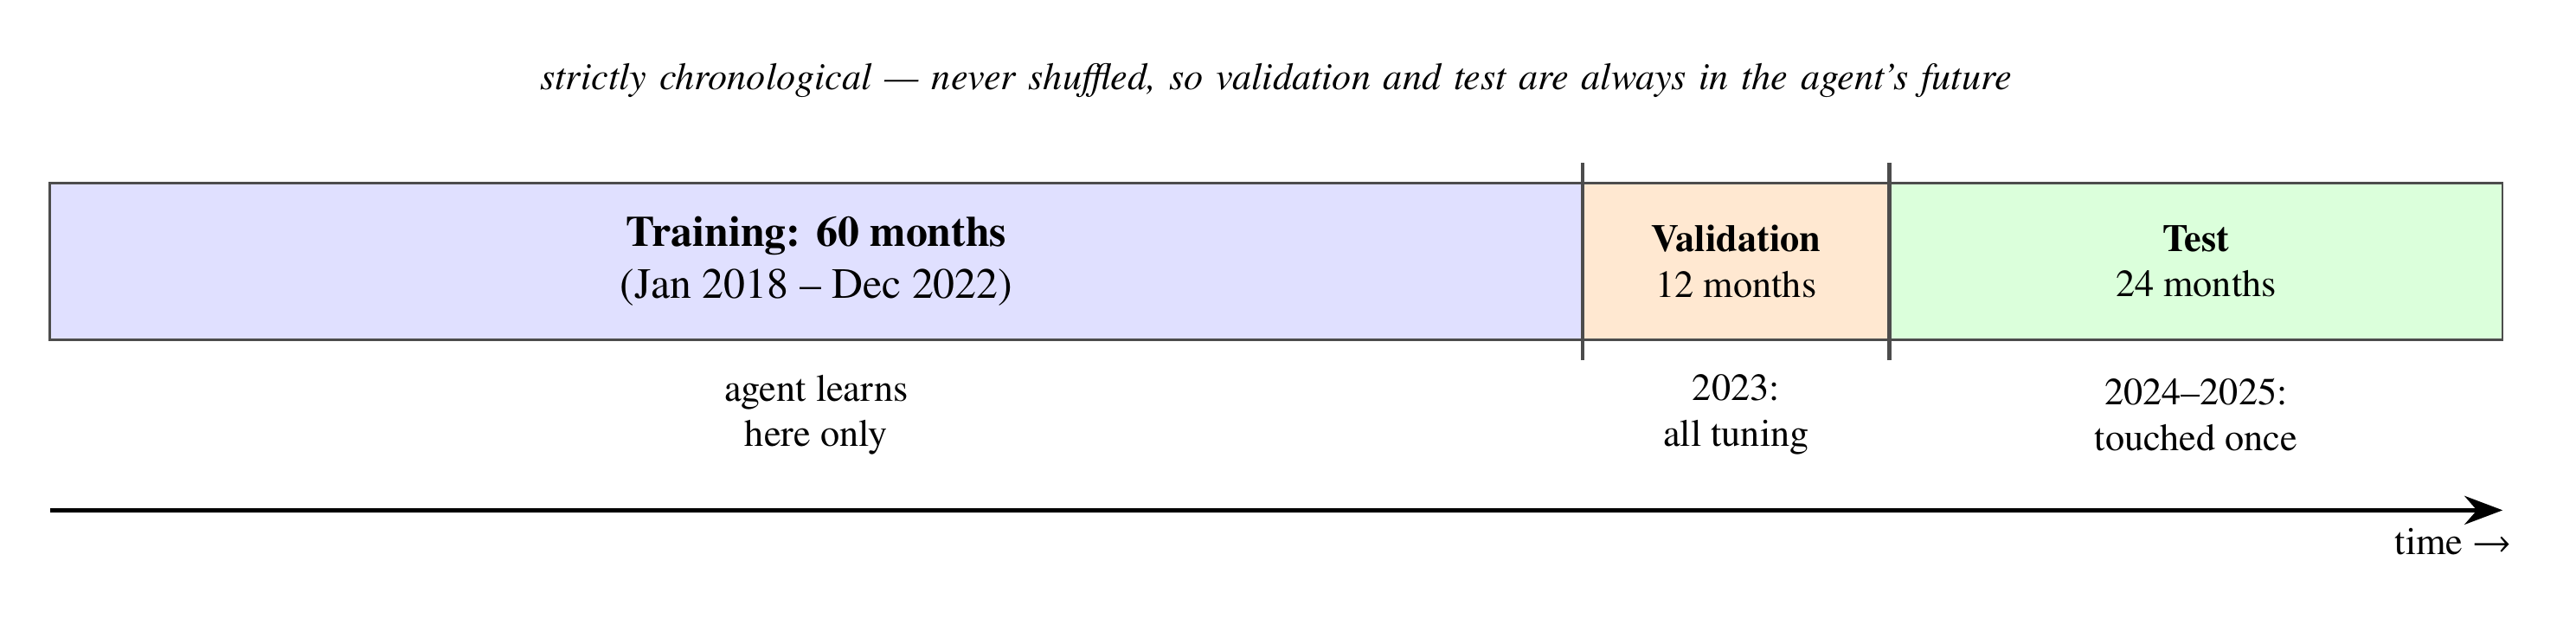
\includegraphics[width=0.9\textwidth]{media4/media/image1.png}
  \caption[Chronological split of the 96 monthly episodes]{Chronological split of the 96 monthly episodes: 60 training months, 12 validation months, and 24 held-out test months.}
\end{figure}


The episodes are kept in chronological order within the splits and are
not randomly shuffled between the three periods. The training set covers
January 2018 to December 2022 (60 monthly episodes) and is used to learn
the algorithms' parameters. The validation set covers 2023 (12 months)
and is used for decisions made during development, such as the fixed
trading amount. The test set contains the final 24 months, January 2024
to December 2025, and is kept separate from these decisions for only the
final evaluation.

Maintaining a chronological split is important for financial data~\cite{lopezdeprado2018}. This
prevents observations from later periods from entering the training set
and influencing the model's development. This would not reflect how a
trading strategy would be developed in practice.

The training period includes most market conditions, including the
volatility experienced in 2018, the COVID-19 market crash and recovery
in 2020, and the 2022 downtrend. The 2023 period is used for validation,
while 2024 and 2025 form the final test period.

The separation between validation and test data is especially important
for the experiments in Chapter 5. A configuration that performs well on
the validation period may therefore be selected to examine its
performance on the held-out test period. The test results are then used
to compare the learned strategies.

The processed episodes and their metadata are cached locally so that the
same dataset can be used consistently across all experiments.

\section{Training, Validation and Testing Procedure}

The experiments use a fixed sequence that separates training,
validation, and test periods. This separation ensures that the test data
are not used when making decisions about the model or experimental
setup.

\subsection{Training}

During training, each learning algorithm interacts with the monthly
episodes in the training period. Each algorithm is given the same market
data, state representation, portfolio conditions, and trading
constraints. The main difference between the algorithms is how they use
the collected experience to update their parameters.

REINFORCE updates the policy using the reward-to-go calculated from
completed monthly episodes. DQN updates its Q-network using transitions
sampled from the replay buffer. PPO collects fixed-length rollouts and
uses the resulting batches for several optimisation epochs.

Each configuration is trained using six random seeds. Using multiple
seeds reduces the dependence on using one particular network
initialisation or a sequence of sampled experiences and allows the variation between runs to be reported~\cite{henderson2018}.

The trained model from each seed is saved with its configuration so that
it can be evaluated later using the same settings.

\subsection{Validation}

The validation set contains the 12 monthly episodes from 2023.

This period is used for decisions that need to be made before the final
test. For example, it determines the fixed transaction amount traded for
each Buy or Sell action.

The candidate transaction sizes are 0.05, 0.10, 0.25, and 0.50 of the
initial capital.

The selection is based on the maximum portfolio exposure that can be
achieved from each action rather than on trading performance during the
test period. This prevents the action from being chosen simply because
it happens to perform well on the final evaluation data.

Once the required configuration decisions have been made, the selected
settings are fixed for testing.

\subsection{Testing}

The final evaluation uses the held-out data from January 2024 to
December 2025.

The test data are not used to make configuration decisions. This ensures
that results provide an independent assessment of the methods.

Each trained model is evaluated in the same trading environment and
using the same evaluation procedure, which includes the initial capital,
transaction costs, action constraints, and monthly episode structure.

For the learned agents, actions are selected intentionally by choosing
the highest-probability action for the policy-based methods or the
highest-valued action for DQN.

The portfolio outcomes are then recorded for each monthly test episode
and each random seed. This produces a consistent set of results that can
be used to compare the different learning algorithms.

The stored results therefore contain sufficient information to compare
algorithms, state representations, reward functions, and benchmark
strategies, which are presented in Chapter 5.

\section{Experiment Configuration}

The implementation was designed so that different experiments could be
run by changing their settings without changing the overall trading
environment or learning algorithm settings.

For this reason, experiments are defined through configuration files or
parameters rather than by manually changing the source code for each
run. Each experiment is therefore linked to a specific configuration
that records the conditions used to produce it.

This separates experiment settings from the environment's implementation
and learning algorithms, allowing the same code to run different state,
reward, and action configurations.

\subsection{Configuration Parameters}

The configuration records the main settings that can affect an
experiment\textquotesingle s outcome. These include:

\begin{itemize}
\item
  learning algorithm;
\item
  state representation and state dimensionality;
\item
  reward formulation;
\item
  transaction fee;
\item
  fixed transaction amounts;
\item
  risk-penalty coefficient, where applicable;
\item
  action model;
\item
  random seed;
\item
  training settings;
\item
  evaluation settings.
\end{itemize}

Using this approach reduces the need to manually change the source code
between experiments. It also makes the experimental process easier to
track, since each result can be linked directly to the configuration
that produced it.

This is particularly important for the experiments reported in Chapter
5, where several state, reward, and action configurations are compared.

\subsection{Algorithm Configuration}

The experiment uses the same starting capital and transaction cost
across all three learning algorithms. The initial capital is set to
\(C_{0} = \$ 10,000\), and a transaction fee of 0.05\% is applied to
each trade opened.

The main settings used for REINFORCE, DQN, and PPO are shown below.

{\def\LTcaptype{none} % do not increment counter
\begin{longtable}[]{@{}
  >{\centering\arraybackslash}p{(\linewidth - 6\tabcolsep) * \real{0.1885}}
  >{\centering\arraybackslash}p{(\linewidth - 6\tabcolsep) * \real{0.2837}}
  >{\centering\arraybackslash}p{(\linewidth - 6\tabcolsep) * \real{0.2699}}
  >{\centering\arraybackslash}p{(\linewidth - 6\tabcolsep) * \real{0.2501}}@{}}
\toprule\noalign{}
\begin{minipage}[b]{\linewidth}\centering
\textbf{Parameter}
\end{minipage} & \begin{minipage}[b]{\linewidth}\centering
\textbf{REINFORCE}
\end{minipage} & \begin{minipage}[b]{\linewidth}\centering
\textbf{DQN}
\end{minipage} & \begin{minipage}[b]{\linewidth}\centering
\textbf{PPO}
\end{minipage} \\
\midrule\noalign{}
\endhead
\bottomrule\noalign{}
\endlastfoot
Network & MLP with 2 hidden layers of 128

\(d \rightarrow 128 \rightarrow 128 \rightarrow 3\) & MLP with 2 hidden
layers of 128

\(d \rightarrow 128 \rightarrow 128 \rightarrow 3\) & \(MlpPolicy\)

\(d \rightarrow 128 \rightarrow 128\) \\
\rowsep
Activation & tanh & ReLU & \\
\rowsep
Optimiser & Adam & Adam & Adam \\
\rowsep
Learning rate & \(10^{- 3}\) & \(10^{- 3}\) & \({3*10}^{- 4}\) \\
\rowsep
Discount factor \(\gamma\) & 0.99 & 0.99 & 0.99 \\
\rowsep
Replay buffer & --- & 50,000 & --- \\
\rowsep
Batch size & Episode & 64 & 64 \\
\rowsep
Target network update & --- & Every 500 steps & --- \\
\rowsep
Exploration & Policy sampling & \(\epsilon - greedy\) & Policy
sampling \\
\rowsep
\(\epsilon\ schedule\) & --- & 1.0 → 0.05 & --- \\
\rowsep
PPO clipping & --- & --- & 0.2 \\
\rowsep
GAE & --- & --- & 0.95 \\
\rowsep
PPO epochs & --- & --- & 10 \\
\rowsep
Entropy coefficient & --- & --- & 0 \\
\rowsep
Training budget & 80,000 steps & 80,000 steps & 80,000 steps \\
\rowsep
Random seeds & 42--47 & 42--47 & 42--47 \\
\end{longtable}
}

All three methods use the same training budget of 80,000 steps and the
same six random seeds to keep the computational budget similar
throughout when comparing performance.

The experiments consider the different state and reward configurations
described in Chapter 5. These include the standard nine-feature state,
the ten-feature state with drawdown, the primary wealth-change reward,
the risk-aware reward, and the alternate action configurations.

The implementation also treats each trading position size as a
configurable parameter. Its final value is selected using the predefined
validation procedure. Chapter 5 reports the different values and their
effect on trading results as part of the experimental findings.

\subsection{Benchmark Implementation}

The learned agents are compared with benchmark strategies to provide
clear grounds for assessing their performance. These benchmarks are
simple trading behaviours that do not require reinforcement learning.

The main benchmark is a buy-and-hold strategy where the initial capital
is used to purchase the asset at the start of the episode. The position
is then held until the final trading step, when it is closed. The same
transaction fee and position closure used for the learned agents apply
to this benchmark.

This approach is different from gradually purchasing the asset using the
same fixed trade amount available to the learning agents. A gradual
purchasing strategy may take several trading days to build a position
and, if the fixed trade size is small, it may not become fully invested
before the monthly episode ends.

For this reason, the gradual purchase strategy is treated as a separate
reference strategy rather than as buy-and-hold. The conventional
buy-and-hold strategy gives the learned agents a straight performance
target.

The benchmark strategies use the same portfolio conditions, transaction
costs, and evaluation procedures as the learned agents. This keeps the
comparison consistent and reduces the chance that differences in results
stem from inaccuracies in calculating portfolio performance rather than
from the strategies themselves.

\section{Implementation Verifications}

Before using the experimental results for analysis, the implementation
was tested to ensure that it followed the definitions and constraints
established in Chapter 3.

These tests check that the environment, data pipeline, reward
calculation, and action constraints behave as intended.

The final implementation includes 21 automated tests covering all major
components, all of which pass. Appendix A lists every test and the
condition it verifies; this section summarises what each group of tests
protects.

\subsection{Environment and Portfolio Tests}

The environment tests focus on the correctness of the portfolio
calculations during trading.

The tests verify that portfolio wealth matches the cash balance and the
market value of current holdings. They also check that Buy and Sell
actions update the portfolio correctly and that transaction fees are
included in all transactions.

The tests further verify that invalid actions are handled correctly and
that each monthly episode ends without an open position.

These checks are important because an error in portfolio accounting
would affect the reported rewards and performance measures for all three
learning algorithms. Such an error could therefore lead to incorrect
conclusions even if the learning algorithms were implemented correctly.

\subsection{Feature and Data Tests}

The feature tests check that the state representation follows the
intended information structure defined in Chapter 3.

The tests verify that features do not use future information and that
rolling features access the necessary historical information when moving
from one monthly episode to the next. They also check that the state
dimensions and feature ordering match the reported configurations.

The chronological split is tested to ensure that the training,
validation, and test periods remain separate.

This testing process identified an important implementation issue. In an
earlier version of the pipeline, rolling features were recalculated
separately for each monthly episode, so the rolling windows restarted at
the beginning of every month instead of continuing from the previous
observations. This caused incomplete feature windows in approximately
\textbf{43.1\% of episode steps}. The correction --- calculating rolling
market features on the continuous dataset before dividing it into
monthly episodes --- is described with the other corrections in Section
4.6, and the corrected pipeline was tested again to confirm that
historical information is retained across episode boundaries.

\subsection{Reward and Risk Tests}

The reward tests verify that the primary wealth-change reward
corresponds to the change in portfolio wealth with no risk penalty
applied.

The risk-aware reward is tested separately to see whether increasing
drawdown does not lead to an increase in the reward due to the risk
penalty applied.

An additional test checks the relationship between the risk-aware reward
and the state representation. A risk-aware reward cannot be paired with
a state that does not have the drawdown feature.

The implementation uses this restriction so an inconsistent combination
of state and reward settings cannot run accidentally.

These tests therefore ensure that the relationship between state
representation and reward design described in Chapter 3 is also
maintained in the implemented system.

\subsection{Action-Masking Tests}

The action-masking tests verify that the environment correctly
identifies invalid actions that cannot be executed under the current
portfolio conditions.

The tests check that the Buy action is unavailable when the portfolio
has insufficient cash and that the Sell action is unavailable when the
agent does not hold enough of the asset. They also verify the different
configurable fixed trading amounts.

A defensive check is also included in the environment so that an invalid
action supplied externally is converted to Hold rather than being
executed.

Logs monitor these checks during the experiments. After the final
experiment, the recorded rate of invalid actions was zero during
evaluation, confirming that the action masks accurately prevented the
learning algorithms from executing any invalid trades during the testing
period.

\section{Implementation Corrections}

\subsection{Problems Identified During Development}

The verification process identified several implementation issues before
the final experiments were run.

The main issues involved the feature calculation, benchmark
implementation, and the risk-aware reward configuration.

First, the rolling market features using past observations did not
initially contain the needed historical context when a new monthly
episode began. These meant that some features were calculated using
shorter windows than intended.

Second, an earlier version of the buy-and-hold benchmark used the same
transaction size as the learning algorithms. This did not represent a
fully invested buy-and-hold strategy, where an asset is bought at the
beginning of an episode and held untouched till the end of the
experiment, and it caused understated exposure and benchmark
performance.

Third, the risk-aware reward could initially be used without requiring
the drawdown feature in the state. This created a mismatch between the
information needed by the reward and the information supplied to the
agent because drawdown information was unavailable.

These issues were treated as implementation errors that needed
correcting because leaving any of them in place would affect the
validity of comparisons between the learning algorithms and benchmark
strategies.

\subsection{Correction and Re-verification}

Each identified issue was addressed through a general correction
process:

\begin{enumerate}
\def\labelenumi{\arabic{enumi}.}
\item
  the problem was identified through testing or auditing the
  implementation;
\item
  its potential effect on the experiment results;
\item
  the relevant part of the implementation that needed correcting;
\item
  adding or updating verification tests where necessary after the
  correction;
\item
  completely running the verification tests again.
\end{enumerate}

The buy-and-hold issue, for example, shows why this process was
necessary. The affected implementation understated the benchmark by
approximately \textbf{\$38.95 per month}, or \textbf{21.6\%} before
correction.

These values describe only the incorrect implementation, which has been
discarded, and are reported here only to show the potential impact of
the error. They are not presented as findings about the
asset\textquotesingle s or the market\textquotesingle s performance.

After the corrections, the complete automated batch tests were run
again, and all 21 tests passed.

The final experiment results in Chapter 5 come only from the corrected
implementation, not the earlier incorrect versions.

\section{Complete Implementation Pipeline}

The complete implementation pipeline is a sequence of stages, from
collecting historical market data to storing the final evaluation test
results.

The first stage loads the SPY OHLCV data, including an initial warm-up
period needed to calculate the rolling features. The market features are
then calculated on the continuous dataset using only information
available up to said observation. Once feature construction is complete,
the data are divided chronologically into the training, validation, and
test datasets.

The observations are then grouped into monthly episodes. At the start of
each episode, the portfolio resets to the initial capital with no asset
holdings. At each timestep, the learning algorithm receives the current
state and selects one of the valid available actions. The trading
environment then executes the action with the transaction fee, updates
the portfolio, returns the reward, and moves to the next state.

REINFORCE, DQN, and PPO all interact with the same trading environment.
Their main difference is how each algorithm processes the experience to
update their model parameters.

After training and validation, the final experiment settings are fixed,
and the trained models are evaluated on the held-out 2024-2025 test
datasets. The resulting metrics, monthly results, training information,
configuration settings, and performance measures are stored together
with information about the software environment used to produce them.

This pipeline clearly links the methodological decisions defined in
Chapter 3, their implementation in the system, and the experiment
results presented in Chapter 5.

Figure 4.2 summarises the flow.

\begin{figure}[!htb]
  \centering
  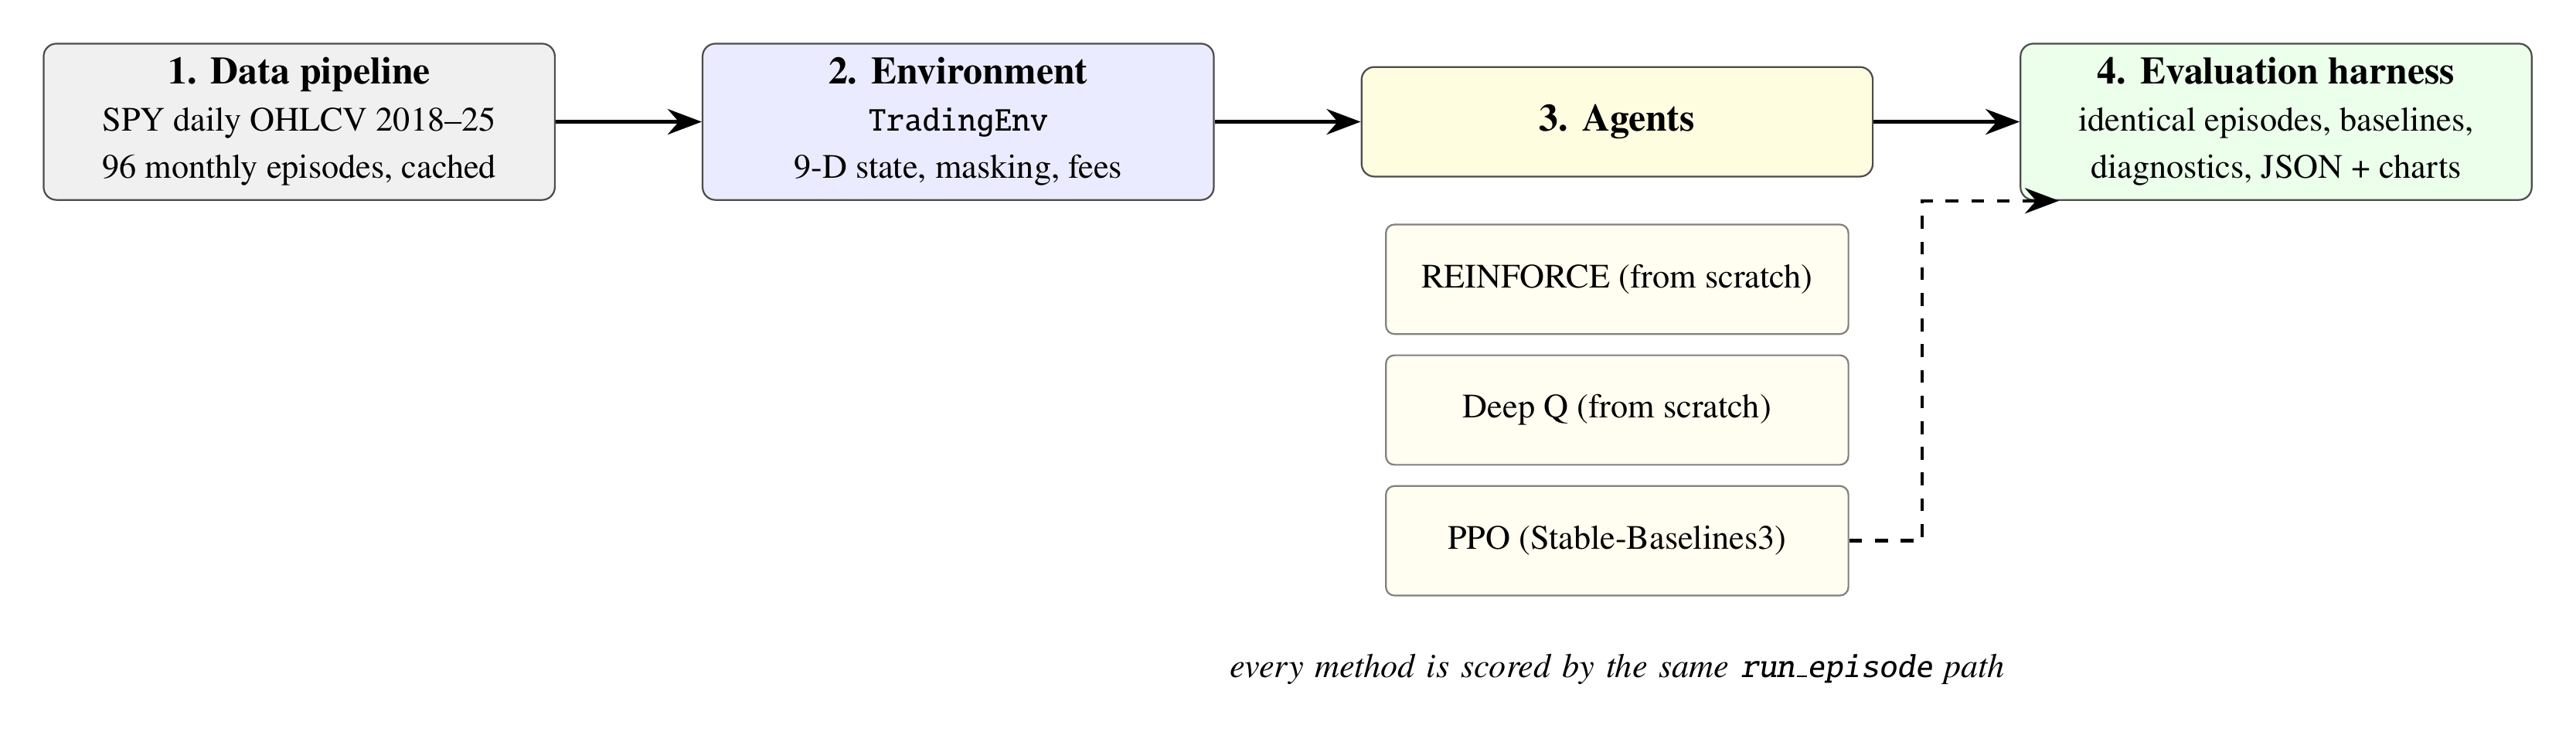
\includegraphics[width=0.9\textwidth]{media4/media/image2.png}
  \caption[System architecture showing the data flow described in Section 4.7.]{System architecture showing the data flow described in Section 4.7. All learned algorithms and benchmark strategies are evaluated using the same episode runner, ensuring that the comparison uses the same evaluation procedure\textbf{.}}
\end{figure}

